\pagestyle{scrheadings}
\ihead[]{\rightmark}
\ohead[]{Iván Rodríguez Méndez}
\ofoot[]{\thepage{}}
\chapter{Introducción}\label{ch:capitulo1}

\section{Objetivos del proyecto}
Los objetivos principales de este proyecto son los siguientes:
\begin{itemize}
	\item Estudio de los distintos filtros de Kalman y los principios básicos de funcionamiento de cada uno de estos para la localización de un robot móvil en suelo deslizante. Los filtros a estudiar serán los siguientes:
    \begin{itemize}
    \item \ac{KF}
    \item \ac{EKF}
    \item \ac{UKF}
    \item \ac{CKF}
    \end{itemize}
    \item Implementación en \textit{MATLAB} de simulaciones para comparar el desempeño de cada uno de los filtros en distintas trayectorias y condiciones. Para la implementación de las simulaciones usaremos una \textit{toolbox} \cite{toolbox_simo} que implementa todos los filtros necesarios dentro de \textit{MATLAB}.
% * <amorellg@ull.edu.es> 2016-05-24T16:44:15.292Z:
%
% > usaremos una
%
% "usaremos y extenderemos una toolbox...", y aquí referencia a la web/publicación de la toolbox
%
% ^.
    \item Simulación en un entorno 3D por medio de una API con el software \textit{V-REP} de la implementación de los filtros en un robot móvil diferencial.
    \item Obtención de conclusiones usando el marco experimental desarrollado por medio de experimentos en las distintas plataformas sobre qué filtro presenta una mejor estimación de la localización del robot.
% * <amorellg@ull.edu.es> 2016-05-24T16:47:44.514Z:
%
% > Conclusión
%
% "Obtención de conclusiones usando el marco experimental desarrollado"
%
% ^.
\end{itemize}
\section{¿Qué es la robótica?}

El término robot fue inventado en 1921 por el novelísta Checo Karel Capek \cite{capek_r.u.r._2004}, para describir unas máquinas inteligentes parecidas a los humanos que realizaban trabajos que estos no podían hacer o que bien no les gustaba hacer. En los años 40, Isaac Asimov acuñó el término robótica y enunció las famosas 3 leyes de la robótica, concretamente en su obra \textit{I, Robot} \cite{asimov_yo_2004}. Las tres leyes son las siguientes \cite{tres_2016}: 
% * <amorellg@ull.edu.es> 2016-05-23T19:34:26.484Z:
%
% > también conocida como \textit{Yo, robot}
%
% Esto lo quitaría
%
% ^ <amorellg@ull.edu.es> 2016-05-23T19:35:38.518Z:
%
% Es más, lo más correcto sería poner además la referencia del libro ;)
%
% ^ <alu0100765755@ull.edu.es> 2016-05-24T09:38:26.266Z:
%
% Puse una referencia aunque no al libro original. Espero que valga !
%
% ^ <alu0100765755@ull.edu.es> 2016-05-24T09:45:15.583Z.

\begin{enumerate}
\item Un robot no hará daño a un ser humano o, por inacción, permitir que un ser humano sufra daño.
\item Un robot debe obedecer las órdenes dadas por los seres humanos, excepto si estas órdenes entrasen en conflicto con la 1ª ley.
\item Un robot debe proteger su propia existencia en la medida en que esta protección no entre en conflicto con la 1ª o la 2ª ley.
\end{enumerate}

Desde entonces la robótica se ha convertido en una importante disciplina científica sobre la que se ha investigado durante décadas. Aunque los mayores avances en este campo se han dado a partir de los años 70 en adelante, al igual que muchas otras ramas de la ciencia, la robótica ha evolucionado casi al mismo tiempo que lo han hecho los sistemas computacionales.
% * <amorellg@ull.edu.es> 2016-05-23T19:36:40.339Z:
%
% > al igual que muchas otras ramas de la ciencia
%
% Te cambié de posición esta frase
%
% ^ <alu0100765755@ull.edu.es> 2016-05-24T09:38:39.311Z:
%
% Ok ! :) 
%
% ^ <alu0100765755@ull.edu.es> 2016-05-24T09:45:18.800Z.

\section{Incertidumbre en sistemas reales}

Podemos definir la robótica como la ciencia relacionada con la percepción e interacción con el entorno por medio del control de dispositivos mecánicos gracias a un ordenador o algún tipo de sistema computacional \cite{thrun_probabilistic_2005}. Algunos ejemplos de éxito relacionado con los sistemas robóticos podrían ser las plataformas de exploración planetaria, brazos robóticos en cadenas de montaje, navegación autónoma de coches en autopistas o por ejemplo drones de rescate para facilitar a los equipos de búsqueda el desempeño de su labor.
% * <amorellg@ull.edu.es> 2016-05-23T19:39:30.481Z:
%
% >  brazos robóticos
%
% un segundo ejemplo con brazos no queda muy bien, pondría un ejemplo de un drone de rescate o algo así
%
% ^ <alu0100765755@ull.edu.es> 2016-05-24T09:39:34.163Z.
% * <amorellg@ull.edu.es> 2016-05-23T19:38:58.057Z:
%
% >  y la manipulación del entorno 
%
% lo cambiaría por "e interacción con el entorno"
%
% ^ <alu0100765755@ull.edu.es> 2016-05-24T09:43:03.767Z.
La realidad es que la mayoría de sistemas robóticos se encuentran aún en su \emph{infancia}, sin embargo la idea de dotar de  ``inteligencia'' a los sistemas robóticos tiene un enorme potencial para cambiar la sociedad. Ideas como evitar los accidentes de tráfico haciendo que los vehículos se comuniquen entre ellos o que incluso lleguen a llevar a las personas de un lugar a otro sin más intervención del factor humano más que para definir el destino al que queremos llegar. Por otro lado también podríamos disponer de sistemas domésticos que se encargaran de las arduas tareas del hogar. Algunos de estos sistemas están bastante extendidos en el mercado, como en el caso del Roomba , un robot capaz de aspirar nuestro hogar localizándose de manera autónoma dentro de este.
% * <amorellg@ull.edu.es> 2016-05-10T15:51:28.343Z:
%
% > Por otro lado también podríamos disponer de sistemas domésticos que se encargaran de las arduas tareas del hogar.
%
% en esto ya podrías poner ejemplos de las aspiradoras robóticas que hay en el mercado, las romba, neato...
%
% ^ <alu0100765755@ull.edu.es> 2016-05-11T12:28:03.912Z.
% * <amorellg@ull.edu.es> 2016-05-10T15:50:44.127Z:
%
% > sistemas de manipulación
%
% no me termina de cuadrar que enlaces esto con las ideas generales de sistemas inteligentes que nombras después
%
% ^ <alu0100765755@ull.edu.es> 2016-05-15T15:41:44.094Z.
% * <amorellg@ull.edu.es> 2016-05-10T15:47:39.568Z:
%
% > ``inteligencia''
%
% en lugar de comillas, considera enfatizar texto con el entorno \emph{}, que lo pone en cursiva
%
% ^ <alu0100765755@ull.edu.es> 2016-05-11T12:29:42.591Z.
% * <amorellg@ull.edu.es> 2016-05-10T15:46:48.834Z:
%
% > ``infancia''
%
% las comillas en latex se ponen de esa manera por defecto, revisa en el resto del texto por si has introducido otra
%
% ^ <alu0100765755@ull.edu.es> 2016-05-15T15:42:01.782Z.

Las aplicaciones de los robots actuales son distintas a los robots del pasado, como por ejemplo, los manipuladores disponibles en las cadenas de montaje que resuelven el mismo problema de forma repetitiva día tras día (típicos de las primeras aplicaciones de la robótica) o en la actualidad aquellos que son capaces de actuar según la variación del propio entorno. La característica más relevante de los nuevos sistemas robóticos es que cada vez son más capaces de trabajar en entornos no estructurados, es decir entornos impredecibles donde no sabemos con qué puede encontrarse el robot. Para ilustrar lo anterior con un ejemplo, podríamos decir que un entorno industrial como una cadena de montaje es bastante más predecible y controlable que un entorno en el interior de una casa. Como resultado, debemos dotar a nuestro robot de un sistema sensorial que sea capaz de interaccionar de alguna manera con el entorno en el que se encuentre y además debe contar con un software lo suficientemente robusto para tomar decisiones de mayor o menor complejidad con diferentes situaciones que se le puedan presentar a este, para que sea capaz de anticiparse a situaciones cambiantes en entornos dinámicos. Por esta razón con el paso de los años la robótica se ha ido transformando y el software se ha convertido en el aspecto más importante de esta rama de la ingeniería. Por ello desarrollar un software robusto y que permita a un robot enfrentarse a entornos dinámicos es un tópico donde actualmente se están invirtiendo grandes esfuerzos en investigación.
% * <amorellg@ull.edu.es> 2016-05-23T19:45:48.582Z:
%
% > tan
%
% lo cambiaría por "es un tópico donde actualmente se están invirtiendo grandes esfuerzos en investigación"
%
% ^ <alu0100765755@ull.edu.es> 2016-05-24T09:46:14.376Z.
% * <amorellg@ull.edu.es> 2016-05-23T19:44:34.366Z:
%
% > muchas de las veces el robot deberá ser capaz de anticiparse a ciertas situaciones
%
% lo cambiaría por "para que sea capaz de anticiparte a situaciones cambiantes en entornos dinámicos"
%
% ^ <alu0100765755@ull.edu.es> 2016-05-24T09:51:12.809Z.
% * <amorellg@ull.edu.es> 2016-05-23T19:43:50.703Z:
%
% > lidiar
%
% lo cambiaría por "tomar decisiones de menor o mayor complejidad"
%
% ^ <alu0100765755@ull.edu.es> 2016-05-24T09:59:01.928Z.
% * <amorellg@ull.edu.es> 2016-05-23T19:41:59.992Z:
%
% > impactante
%
% pondría "relevante"
%
% ^ <alu0100765755@ull.edu.es> 2016-05-24T09:59:17.975Z.
% * <amorellg@ull.edu.es> 2016-05-10T15:52:54.334Z:
%
% > desestructurados
%
% "no estructurado" es el término más habitual
%
% ^ <alu0100765755@ull.edu.es> 2016-05-15T15:44:30.771Z.
% * <amorellg@ull.edu.es> 2016-05-10T15:52:15.318Z:
%
% > Las aplicaciones de los robots del mañana son distintas a los robots del pasado
%
% poético!! pero no le encuentro mucho sentido, me lo tendrás que explicar!
%
% ^ <alu0100765755@ull.edu.es> 2016-05-15T15:50:54.842Z:
%
% Habrá que intentar explicar mejor esta idea veremos si es posible.
%
% ^ <alu0100765755@ull.edu.es> 2016-05-24T10:03:00.036Z.
% * <amorellg@ull.edu.es> 2016-05-10T15:49:28.959Z:
%
% > recursiva
%
% "recursividad" no sería eso exactamente, imagino que pensaba en "repetitiva"
%
% ^ <alu0100765755@ull.edu.es> 2016-05-15T15:53:10.047Z.

El punto central de este trabajo no es otro que la \textbf{estimación de estados con incertidumbre}. Este será un punto clave ya que necesitamos saber donde se encuentra el robot en cada instante y para nosotros no será lo mismo que  el robot se encuentre a 1 metro del objetivo que a 5 metros. Es obvio que cuanta más certeza tengamos en las estimaciones, menos incertidumbre encontraremos sobre las variables que queremos conocer y mejor será el funcionamiento de nuestro sistema. Para tratar este problema tenemos una serie de aspectos que influyen en el rendimiento de un estimador de estados, son los siguientes:
% * <amorellg@ull.edu.es> 2016-05-10T15:56:31.684Z:
%
% > Para tratar este problema tenemos cinco factores que se postulan como los más influyentes, son los siguientes:
%
% me suena rara esta frase, más bien "una serie de aspectos que influyen en el rendimiento de un estimador de estados", o algo así
%
% ^ <alu0100765755@ull.edu.es> 2016-05-15T15:58:08.058Z.
% * <amorellg@ull.edu.es> 2016-05-10T15:54:30.397Z:
%
% >  punto central 
%
% estimación de estados con incertidumbre diría yo
%
% ^ <alu0100765755@ull.edu.es> 2016-05-15T15:59:12.687Z.

\begin{enumerate}
 \item \textbf{Entorno}: Es lógico pensar que el mundo, es decir el entorno, es un lugar impredecible donde no podemos saber que se encontrará el robot. A pesar de lo anterior pueden llegar a existir entornos donde esa incertidumbre esté controlada, como los entornos industriales, o por el contrario donde muchos factores son impredecibles como podrían ser las carreteras o los hogares.
 \item \textbf{Sensores:} Cuentan con la limitación con respecto a la información que pueden percibir de su entorno. Las limitaciones derivan de dos factores principales, el primero de ellos está relacionado con el rango y la resolución de estos lo cual está sujeto a variables físicas. Un ejemplo claro es que las cámaras no pueden ver a través de una pared, incluso cuando no tienen ningún elemento que dificulte su percepción, la propia resolución espacial de la cámara está limitada. En segundo lugar, los sensores están siempre sujetos a ruidos que perturban las medidas de forma aleatoria (más adelante veremos como podemos modelar el ruido para su compensación) lo cual limita en gran medida la información que somos capaces de obtener de ellos.
% * <amorellg@ull.edu.es> 2016-05-10T16:00:07.731Z:
%
% > de formas impredecibles
%
% se pueden predecir de cierta forma, de ahí que funcionen los filtros bayesianos... ;D más bien, ruido que es necesario modelar para intentar compensar
%
% ^ <alu0100765755@ull.edu.es> 2016-05-15T16:03:24.240Z:
%
% Menudo fallo !! :O Vamos a cambiarlo rápidamente !
%
% ^ <alu0100765755@ull.edu.es> 2016-05-15T16:52:56.736Z.
 \item \textbf{Actuadores}: Las acciones desarrolladas por los robots se dan en su mayoría por medio de motores y la gran parte de ellos pueden introducir efectos impredecibles como el control del ruido introducido en la consiga o incluso el desgaste de rodamientos y uniones (lo que provoca un comportamiento no deseado). Sin embargo en el mercado existen muchos tipos de actuadores, algunos como los de los robots industriales para trabajos pesados son precisos en cuanto a sus movimientos, por otra parte los actuadores con los que cuentan los robots de bajo coste son bastante imprecisos. De esta manera la construcción y las características de nuestro robot también podrían influir en la incertidumbre que tengamos.
% * <amorellg@ull.edu.es> 2016-05-10T16:01:54.906Z:
%
% > bastante exactos
%
% es más técnico si dices "repetibilidad"
%
% ^ <alu0100765755@ull.edu.es> 2016-05-15T16:08:22.313Z:
%
% Creo que el término que buscaba era "precisos"
%
% ^ <alu0100765755@ull.edu.es> 2016-05-15T16:52:54.484Z.
% * <amorellg@ull.edu.es> 2016-05-10T16:01:29.010Z:
%
% > Robots
%
% aquí quieres decir "Actuadores", no?
%
% ^ <alu0100765755@ull.edu.es> 2016-05-15T16:52:53.544Z.
 \item \textbf{Modelos}: Los modelos son imprecisos, este hecho es inevitable. No debemos pasar por alto que los modelos no son más que meras abstracciones del mundo real. Como tal estos solo caracterizan el proceso físico que tiene lugar entre el robot y su entorno. Los errores en el modelo son otra fuente de incertidumbre, y además es una de las cuestiones que más se ha pasado por alto en robótica a pesar de que la mayoría de modelos existentes en el estado del arte son en su mayoría muy simplificados.
% * <amorellg@ull.edu.es> 2016-05-10T15:56:12.413Z:
%
% >  Los modelos suelen ser muchas veces imprecisos
%
% muchas veces no, siempre!!!
%
% ^ <alu0100765755@ull.edu.es> 2016-05-15T16:52:52.317Z.
 \item \textbf{Computación}: Los robots son sistemas de tiempo real y por lo tanto están limitados con respecto a la cantidad de recursos computacionales disponibles para ejecutar órdenes en un instante de tiempo (siempre y cuando nos estemos refiriendo a robots que interactúan en tiempo real con el entorno para adaptarse a los cambios ocurridos en él). La mayoría de algoritmos disponibles con mejor rendimiento (incluido el filtro de Kalman, que estudiaremos más adelante) parten de ciertas simplificaciones para ahorrar recursos computacionales, lo cual empeora la precisión de nuestro sistema.
% * <amorellg@ull.edu.es> 2016-05-10T16:05:23.617Z:
%
% >  estado del arte
%
% ojo con esta expresión porque es una traducción literal y no debería usarse de esta manera (aunque todos lo hagamos...), intenta decirlo de otra manera, como "los disponibles con mejor rendimiento", o "desempeño".... 
%
% ^ <alu0100765755@ull.edu.es> 2016-05-15T16:15:16.795Z:
%
% Buen consejo! Así no cometo el mismo error más adelante 
%
% ^ <alu0100765755@ull.edu.es> 2016-05-15T16:52:49.320Z.
% * <amorellg@ull.edu.es> 2016-05-10T16:04:06.361Z:
%
% > Los robots son sistemas de tiempo real y por lo tanto están limitados con respecto a la cantidad de recursos computacionales disponibles para ejecutar órdenes en un instante de tiempo.
%
% sí pero no, un manipulador en una industria no necesita tiempo de cómputo para una tarea repetitiva. Entiendo que te refieres a un robot que interactúa en tiempo real con el entorno adaptándose a cambios a su alrededor
%
% ^ <alu0100765755@ull.edu.es> 2016-05-15T16:52:46.729Z.
\end{enumerate}

Todos estos factores pueden hacer que la incertidumbre aumente. Tradicionalmente no se tenían en cuenta y por lo tanto la incertidumbre era un tema que se solía ignorar ya que el robot actuaba en espacios controlados. La tendencia de cambio en el estudio de la incertidumbre se debe a que cada vez más se necesita que los robots actúen en entornos no estructurados y por lo tanto poder lidiar con ella hará que nuestro robot pueda funcionar de forma correcta.

\section{Robótica probabilística}

Durante el desarrollo de este trabajo trataremos de resolver la localización de nuestro robot por medio de algoritmos que en su fundamentación tienen una base probabilística. La probabilidad en la robótica es un enfoque que nos permite saber cuantificar de alguna forma el grado de incertidumbre tenemos en la percepción de nuestro robot y en sus acciones. Por lo tanto la idea principal de la aplicación de la probabilidad es tener explícitamente datos que nos indiquen cual es la incertidumbre, para ello usamos los cálculos de probabilidades. Otra diferencia la encontramos a la hora de realizar medidas, en lugar de confiar totalmente en la medida que nos devuelve nuestro sensor, lo que harían los algoritmos probabilísticos sería representar esa información por medio de una distribución de probabilidad lo cual nos daría una idea de la incertidumbre sobre nuestra medida. Lo anterior se traduce en que tendremos mayor conocimiento sobre la verosimilitud de nuestras medidas aplicando estos algoritmos. Como ya veremos más adelante la aplicación de algoritmos basados en probabilidades solucionan muchos problemas relacionados con las fuentes de incertidumbre que enumerábamos en el apartado anterior.
% * <amorellg@ull.edu.es> 2016-05-23T19:49:12.781Z:
%
% > transfondo
%
% "fundamentación" ?
%
% ^ <alu0100765755@ull.edu.es> 2016-05-24T10:03:27.099Z.
% * <amorellg@ull.edu.es> 2016-05-10T16:08:57.168Z:
%
% > en lugar de confiar en una sola medida que nos devuelva nuestro sensor lo que harían los algoritmos probabilísticos sería representar la información por medio de una distribución de probabilidad siempre teniendo en cuenta un espacio de posibles hipótesis
%
% esto no me parece acertado al 100% ponerlo así, ya que parece que un sensor te da un rango de valores, cuando sí que es cierto que se sigue considerando una medida, pero se contempla si grado de verosimilitud como comentas
%
% ^ <alu0100765755@ull.edu.es> 2016-05-15T17:06:35.271Z:
%
% Espero que con el cambio quedara mejor :) 
%
% ^ <amorellg@ull.edu.es> 2016-05-23T19:50:47.617Z:
%
% olrait !
%
% ^ <alu0100765755@ull.edu.es> 2016-05-24T10:04:09.454Z.

Para ilustrar mejor el enfoque probabilístico usaremos un sencillo y visual ejemplo: la localización de un robot móvil \cite{thrun_probabilistic_2005}, que además es el tema en el que basamos este trabajo. La localización es el problema de estimar las coordenadas de un robot con respecto a un sistema de coordenadas de referencia con ayuda de los sensores y usando un mapa del entorno en el que se encuentra. Las coordenadas de las que hablamos en nuestro caso corresponden al vector de estados del robot que queremos estimar, las variables especificadas dentro del vector siguiente:
% * <amorellg@ull.edu.es> 2016-05-23T19:51:30.675Z:
%
% > Este ejemplo lo hemos extraído de \cite{thrun_probabilistic_2005}
%
% Esta referencia la pondría directamente tras "robot móvil" justo antes, que básicamente es lo mismo que decir explícitamente que está extraído de ahí
%
% ^ <alu0100765755@ull.edu.es> 2016-05-24T10:06:05.312Z.
\begin{equation}
p = 
\left(
\begin{array}{cccc}
x \\
y \\
\theta 
\end{array}
\right)
\end{equation}
Donde, $x$ corresponde a la localización en dicho eje con respecto al sistema de referencia en metros o la unidad de medida longitudinal que decidamos usar; $y$ sería lo mismo que $x$ pero refiriéndose a su propio eje. Por último $\theta$ se correspondería a la rotación de nuestro robot con respecto a una referencia donde fijaríamos el cero. La unidades son radianes.
% * <amorellg@ull.edu.es> 2016-05-23T19:54:34.378Z:
%
% > La unidades más usadas para medir la rotación son los radianes.
%
% basta con que pongas "en radianes" :)
%
% ^ <alu0100765755@ull.edu.es> 2016-05-24T10:07:13.544Z.
% * <amorellg@ull.edu.es> 2016-05-23T19:53:41.739Z:
%
% > usar. $y$ sería
%
% queda mejor como una secuencia separada por punto y coma para cada explicación
%
% ^ <alu0100765755@ull.edu.es> 2016-05-24T10:10:27.882Z.
% * <amorellg@ull.edu.es> 2016-05-23T19:53:18.387Z:
%
% > Donde
%
% porqué negrita?
%
% ^ <alu0100765755@ull.edu.es> 2016-05-24T10:10:42.978Z.

En la figura \ref{Markov_Localization} podemos ver una ilustración que plasma el enfoque de la localización probabilística para un robot móvil. 
\begin{figure}[t!]
\centering
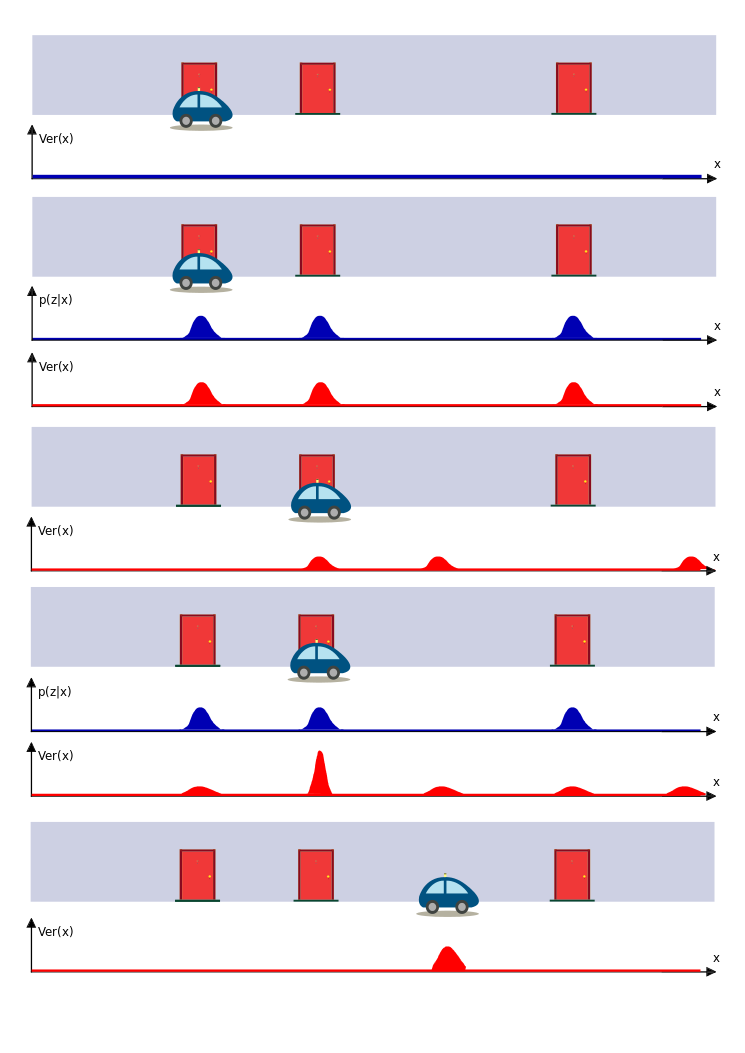
\includegraphics[scale=1]{Localizacion}
\caption{Diagrama de localización de Markov \cite{thrun_probabilistic_2005}.} \label{Markov_Localization}
\end{figure}
El problema de la localización para este ejemplo se conoce
como localización global donde el robot se encuentra en cualquier
punto del entorno y debe localizarse a si mismo desde cero
(sin ningún conocimiento previo de donde puede estar).
Como ya hemos comentado en este tipo de localización
la estimación en un instante de tiempo (también conocida como certidumbre) se representa por medio de una función de densidad de probabilidad que se encuentra distribuida en el espacio en el que realizamos la localización (un entorno tridimensional o bidimensional).
% * <amorellg@ull.edu.es> 2016-05-23T20:14:19.602Z:
%
% > verosimilitud
%
% no es realmente eso, es la medida de lo buena que es esa estimación
%
% ^ <alu0100765755@ull.edu.es> 2016-05-24T10:13:55.809Z:
%
% Creo que el término es certidumbre.
%
% ^ <amorellg@ull.edu.es> 2016-05-24T16:50:22.920Z:
%
% Mejor
%
% ^.
Lo anterior se ilustra en el primer fragmento de la figura \ref{Markov_Localization} donde se muestra una distribución uniforme (a priori) lo cual corresponde a la máxima incertidumbre (coincidiendo con la localización inicial). 
Suponemos entonces que el robot toma una primera medida y el resultado de esta nos dice que el robot se encuentra cerca de una puerta. 
La verosimilitud resultante se muestra en el segundo fragmento de la figura \ref{Markov_Localization} donde podemos observar que los puntos de máxima probabilidad se colocan donde se encuentran las puertas (ya que nuestra medida nos indica que es más probable que estemos en alguno de estos puntos) y en cualquier otro punto tenemos una probabilidad más baja. 
Como podemos ver esta distribución presenta tres picos, cada uno de estos picos corresponden a cada puerta de manera indistinguible por lo que se asigna la misma probabilidad de encontrarse en cualquiera de estos tres lugares.
Además, la distribución de probabilidad asigna alta probabilidad a tres diferentes localizaciones, ilustrando de esta manera que el marco de referencia probabilístico puede tener en cuenta distintas hipótesis que podrían llegar a entrar en conflicto y generar situaciones ambiguas. Finalmente, incluso en los lugares donde no está localizada una puerta tenemos una probabilidad distinta de cero.
% * <amorellg@ull.edu.es> 2016-05-23T20:15:47.921Z:
%
% > lidiar
%
% "hacerse cargo" o "tener en cuenta"
%
% ^ <alu0100765755@ull.edu.es> 2016-05-24T10:16:21.994Z.
Lo anterior es debido a la incertidumbre que tenemos al realizar las medidas, por lo tanto si tenemos una probabilidad pequeña pero distinta de cero tenemos en cuenta la posibilidad de que el robot esté errando y por lo tanto no esté cercano a una puerta. 
% * <amorellg@ull.edu.es> 2016-05-10T16:51:47.093Z:
%
% > lo cual corresponde 
%
% esto está dos veces
%
% ^ <alu0100765755@ull.edu.es> 2016-05-15T17:31:26.958Z.
% * <amorellg@ull.edu.es> 2016-05-10T16:50:19.974Z:
%
% >  las coordenadas de un robot 
%
% en algún sitio estaría bien introducir que "las coordenadas" es el vector de estados de un robot móvil que queremos estimar, y especificar qué estados son, es decir: [x,y,theta]
%
% ^ <alu0100765755@ull.edu.es> 2016-05-15T17:31:38.437Z.
% * <amorellg@ull.edu.es> 2016-05-10T16:14:57.997Z:
%
% > En la figura \ref{Markov_Localization} podemos
%
% esta figura además está como dos páginas después de que hables de ella, no te cortes en ponerla justo tras la frase donde la referencias por primera vez, ya latex se encarga de colocarla en esa página o la siguiente donde mejor cuadre
%
% ^ <alu0100765755@ull.edu.es> 2016-05-15T17:41:11.236Z:
%
% No se como hacer para que latex decida donde ponerla. Se que se hace con un comando pero creo que no está funcionando bien
%
% ^ <alu0100765755@ull.edu.es> 2016-05-15T17:43:49.615Z.
% * <amorellg@ull.edu.es> 2016-05-10T16:11:13.302Z:
%
% > figura
%
% ah vale, esta es la figura que dices que veías pequeña, no?
%
% ^ <alu0100765755@ull.edu.es> 2016-05-15T17:43:59.653Z:
%
% Sep !
%
% ^ <amorellg@ull.edu.es> 2016-05-16T17:11:28.960Z.

Ahora supongamos que el robot se mueve hacia la derecha. El tercer fragmento de la figura \ref{Markov_Localization} muestra lo que le ocurre a la verosimilitud del robot cuando este se mueve, siempre y cuando el movimiento del robot se de tal y como asumimos. Vemos que la verosimilitud se desplaza en la misma medida que el robot, es decir, que se desplaza en la dirección de movimiento de este. También podemos observar como los picos se han suavizado debido a la incertidumbre existente en relación al movimiento del robot, ya que a medida que nos movemos sin volver a medir más estamos aumentando la incertidumbre sobre donde nos encontramos. Para finalizar, en el cuarto fragmento de la figura \ref{Markov_Localization} está presentada la verosimilitud después de realizar la medida y darnos cuenta de que el robot se ha encontrado cerca de otra puerta. Esta observación permite a nuestro algoritmo asignar altas probabilidades de que el robot se encuentre cerca de una de las puertas por lo tanto las probabilidades para cada una de ellas no serán las mismas. Debido a esta segunda medida el robot se ha reducido la incertidumbre en su localización con respecto al momento antes de realizar la medida.
% * <amorellg@ull.edu.es> 2016-05-10T16:56:14.340Z:
%
% > está bastante mejor localizado
%
% yo diría más bien, "se ha reducido la incertidumbre en su localización"
%
% ^ <alu0100765755@ull.edu.es> 2016-05-15T17:45:06.416Z.

Como hemos visto este ejemplo ilustra el paradigma probabilístico en el contexto de aplicación en un problema concreto. El problema de la percepción del robot es un problema en cuanto a la estimación de los estados, y en el ejemplo que hemos mostrado se usa una herramienta conocida en probabilidad como \textbf{filtro bayesiano} o \textbf{teorema de bayes} para la estimación posterior del estado de la localización del robot en el espacio en el que se encuentra. Hablaremos sobre este teorema en posteriores apartados (Capítulo \ref{ch:capitulo2}  y Apéndice \ref{ApendiceA}).
% * <amorellg@ull.edu.es> 2016-05-23T20:19:17.992Z:
%
% > un algoritmo
%
% me suena mejor "una herramienta"
%
% ^ <alu0100765755@ull.edu.es> 2016-05-24T10:29:45.850Z.
% * <amorellg@ull.edu.es> 2016-05-10T16:57:00.539Z:
%
% > sobre este teorema en posteriores capítulos.
%
% poner la referencia cuando sepas el capítulo
%
% ^ <alu0100765755@ull.edu.es> 2016-05-24T10:34:03.354Z:
%
% Parece que ya está !
%
% ^ <alu0100765755@ull.edu.es> 2016-05-24T10:34:08.834Z.

\section{Ventajas y desventajas del enfoque probabilístico}

Llegados a este punto la pregunta más importante probablemente sea cuales son las ventajas de un enfoque probabilístico en comparación a otras aproximaciones que no representan la incertidumbre de forma explícita. La respuesta a esta pregunta es una premisa general que sigue el enfoque que trataremos en este trabajo, y es la siguiente: \textit{Un robot que tiene conocimiento de su propia incertidumbre y actúa en consonancia con esto es superior a otro que no lo hace.}

En general los enfoques probabilísticos son más robustos de cara a las limitaciones que presentan los sensores, es decir, con el ruido que introducen a las medidas, cómo les afecta la dinámica del entorno y demás efectos que se pueden producir sobre estos. Su gran ventaja sobre otras aproximaciones se aprecia cuando se aplica en entornos no estructurados donde la robustez ante la incertidumbre  es tremendamente importante. La realidad es que los algoritmos basados en probabilidades son los únicos que han conseguido trabajar de forma correcta en los problemas más complejos de estimación de  estados en robótica. Un ejemplo muy típico para ilustrar lo anterior es el del \textit{robot secuestrado} donde el robot por sus propios medios debe recuperarse de un fallo de localización. Por contra, los algoritmos basados en probabilidad tienen sus puntos débiles en la precisión de los modelos que utilizan muchos algoritmos clásicos y como ya dijimos esto puede llegar a ser una fuente de incertidumbre.
% * <amorellg@ull.edu.es> 2016-05-10T16:58:45.986Z:
%
% > la habilidad de lidiar con
%
% robustez ante la incertidumbre
%
% ^ <alu0100765755@ull.edu.es> 2016-05-15T17:47:11.506Z.
% * <amorellg@ull.edu.es> 2016-05-10T16:58:14.722Z:
%
% > desestructurados
%
% no estructurados
%
% ^ <alu0100765755@ull.edu.es> 2016-05-15T17:47:13.654Z.

Sin embargo, parece que las ventajas aún son mayores que las desventajas que se presentan. Por lo general, las dos limitaciones más frecuentes citadas de estos algoritmos son la \textbf{ineficiencia computacional}, y que \textbf{necesitan basarse en aproximaciones}. Los algoritmos probabilísticos son en esencia menos eficientes que los que no lo son, debido a que en ellos se consideran densidades de probabilidad completas. Por lo tanto estos modelos necesitan ser aproximados ya que el robot se mueve en un espacio continuo y tratar con los datos de esta manera para un sistema computacional sería casi inviable. Muchas veces la solución se basa en que la incertidumbre puede ser aproximada por medio de un modelo paramétrico compacto (que en nuestro caso será una distribución de probabilidad Gaussiana) por norma general la solución analítica de los modelos suele ser bastante inmanejable o costosa computacionalmente, por lo que se utilizan métodos aproximados que generalmente resuelven un problema de optimización . La utilización de los modelos compactos y las aproximaciones permitirán utilizar estos algoritmos con una eficiencia computacional muy superior.
% * <amorellg@ull.edu.es> 2016-05-10T17:02:20.432Z:
%
% >  y en otros caso las aproximaciones pueden llegar a ser mucho más complicadas que el modelo compacto que usaremos
%
% otra forma más técnica de decirlo es que por norma general la solución analítica de los modelos suele ser bastante inmanejable o costosa computacionalmente, por lo que se utilizan métodos aproximados que generalmente resuelven un problema de optimización
%
% ^ <alu0100765755@ull.edu.es> 2016-05-15T18:09:45.954Z.

\section{Organización del documento}
% * <amorellg@ull.edu.es> 2016-05-23T20:20:58.879Z:
%
% > Organización
%
% Antes de esto faltaría añadir una sección con los objetivos del proyecto (que no recuerdo si lo habíamos hablado ya), sobre todo para aclarar que vas a usar filtros de Kalman, qué piensas obtener con ellos, etc. También para que no se me olvide (que no sé si lo ibas a poner ya en el capítulo 3) habría que nombrar que un filtro de kalman es un estimador de máxima verosimilitud, para la función de densidad de probabilidad de ruido que asuma...
%
% ^.

En este trabajo trataremos de dar una idea general sobre la estimación probabilística y sobre los filtros de Kalman como ejemplo de aplicación. Iremos evolucionando desde una introducción matemática básica para comprender mejor las herramientas de las que disponemos hasta una serie de experimentos donde intentaremos ver que filtro presenta un mejor desempeño cuando lo aplicamos a un robot móvil con deslizamiento. La organización del documento es la siguiente:
\begin{itemize}
\item En el capítulo \ref{ch:capitulo2}, haremos una introducción a los filtros de Kalman y a todos los conceptos básicos.
\item En el capítulo \ref{ch:capitulo3}, introduciremos cada uno de los filtros que estudiaremos en este trabajo además de explicar sus algoritmos de funcionamiento.
\item En el capítulo \ref{ch:capitulo4}, describiremos todas las herramientas y equipos utilizadas para la realización de este trabajo.
\item En el capítulo \ref{ch:capitulo5}, realizaremos los experimentos sobre los filtros y determinaremos cual es el que presenta el mejor comportamiento ante diferentes situaciones de experimentación.
\item Finalizaremos con una conclusión global sobre el trabajo realizado y plantearemos posibles trabajos futuros en la misma línea.

\end{itemize}

% * <amorellg@ull.edu.es> 2016-05-24T16:51:11.344Z:
%
% > En el capítulo \ref{ch:capitulo2}:
% > Descripción de cada capítulo de la memoria: en el capítulo 2 blablaba, en el 3 blabla, en el 4 experimentos....
%
% ojo :)
%
% ^.
